\section{Ursprung}

Wie im Artikel zu \ac{DevOps} auf den Seiten 10 und folgende des Magazins Objektspektrum 06/20 \cite{spektrum1} kurz angesprochen, beruht die Idee von \ac{DevOps} ursprünglich nicht auf Prinzipien aus der IT, sondern Prozessideen aus der industriellen Anfertigung, vor allem aus den Produktionshallen von Toyota. Von dort werden auch die Ansätze des Lean Managements und Kanban genutzt, die beide die Prozesskette als sehr wichtig betrachten und als Grundidee haben, dass sich die einzelnen Teilprozesse untereinander verständigen und abstimmen, um insgesamt den Prozess effizienter und stabiler zu betreiben. Insgesamt ging es bei Toyota damals im Bezug auf die effizientere Gestaltung der Prozesskette darum, alles darauf auszulegen, dass die Zeitspanne zwischen der Erteilung eines Auftrags bis zu dem Zeitpunkt, an dem das Geld fließt, so stark verkürzt wird wie möglich. \cite{halstenberg:2020} Das ist unter anderem durch weglassen unnötigen Aufwands (im japanischen \glqq Muda\grqq\ genannt) und die effizientere Gestaltung einzelner Teilprozesse durch die Nutzung der Ideen von Kanban und Lean zu erreichen. Kanban beschreibt grundsätzlich das Konzept, dass jeder Teilprozess eigenständig seine Produktion verwaltet, d. h. jede Abteilung fordert selbst an, wie viele Ressourcen benötigt werden und auf der anderen Seite produziert jede Abteilung nur genau so viel, wie die folgende Abteilung anfordert. Dadurch wird eine zentralisierte Ressourcenverteilung in den Hintergrund gestellt, und jede Abteilung ist selbst verantwortlich, das sie grundsätzlich am besten weiß, was gerade wie viel benötigt wird \cite{ohno:1988}. Die Ideen des Lean Managements werden in den folgenden Abschnitten angesprochen und vor allem in \autoref{sec:calms} genauer beschrieben.

Das Wort \ac{DevOps} ist das erste Mal während einer Konferenz im Jahr 2009 als Hashtag auf Twitter gestartet. Einige Monate später gab es eine erste Konferenz namens \glqq DevOpsDays\grqq\ in Gent, mit deren Start sich das Konzept von \ac{DevOps} rasant verbreitete \cite{halstenberg:2020}.

\section{Leitsatz}

Auch wenn mit der Philosophie des \ac{DevOps} einige Tools und Methoden gegeben werden, um die Überwindung der Wall of Confusion zu erreichen, so ist \ac{DevOps} doch viel mehr auch eine strukturelle Denkweise, die viel Arbeit braucht, um sie in den Köpfen der Nutzenden zu verankern. Es ist wichtig, sich als Nutzer von \ac{DevOps} immer wieder darauf zurück zu besinnen, dass \ac{DevOps} ein kontinuierlicher Prozess ist, der immer und immer wieder neue und alte Arbeit fordert.

Wie zuvor schon erwähnt ist es wichtig, von der Silodenke wegzukommen und sich und seine Abteilung nicht als eigenen Block zu sehen, der seine Arbeit macht und dann fertig ist, sondern dass man selbst weiß, wo man im Gesamtprozess einzuordnen  ist und wie die eigene Arbeit mit der Arbeit anderer Teilprozesse bzw. Abteilungen zusammenhängt. Unter anderem ist es dafür wichtig zu wissen, was und wie die anderen Teilprozesse arbeiten und was dort als Input bzw. Output erwartet wird. Im Lean Management wird in diesem Zusammenhang von internen und externen Kunden gesprochen. Die externen Kunden sind die klassischen Kunden, die als Außenstehende des Betriebs die Entwicklung eines Produkts in Auftrag geben. Das diese Art Kunde für den Prozess von großem Wert ist, steht außer Frage, da hiermit der zahlende Kunde gemeint ist. Der interne Kunde stellt das weitaus interessanteren Konzept dar, da hiermit alle Parteien gemeint sind, die irgendwie von einem Teilprodukt abhängig sind. Somit sind für einen Teilprozess alle anderen Teilprozesse, die letztendlich das Produkt der Arbeit aus dem Teilprozess erhalten, interne Kunden für diesen Teilprozess und müssen mit Kommunikation in die Arbeit und Gestaltung des Produkts mit eingebunden werden. Ein Team steht somit immer im Kontakt mit Teams, die ihr Produkt weiter verwerten sowie mit Teams, deren Produkte vom eigenen Team weiter verwertet werden. Das ist somit schon ein Konzept, um die Wall of Confusion, wie sie in \autoref{fig:wall} gezeigt wurde, einzureißen. Auch wenn zwei Abteilungen wie Dev und Ops scheinbar völlig entgegengesetzte Ziele erreichen wollen, so wollen alle, dass der Prozess erfolgreich beendet wird und das Produkt an den externen Kunden geliefert wird. Mit der Idee der internen Kunden können dann auch die scheinbar gegensätzlichen Ziele miteinander vereinbart und die Arbeit effizienter gestaltet werden.

Hierfür werden Prinzipien aus der agilen Entwicklung genutzt, unter anderem ein System von Feedforward und Feedback in kurzen Zyklen zwischen den beiden Abteilungen Dev und Ops, wie es in \autoref{fig:schleife} grob dargestellt ist.

\begin{figure}[h]
\centering
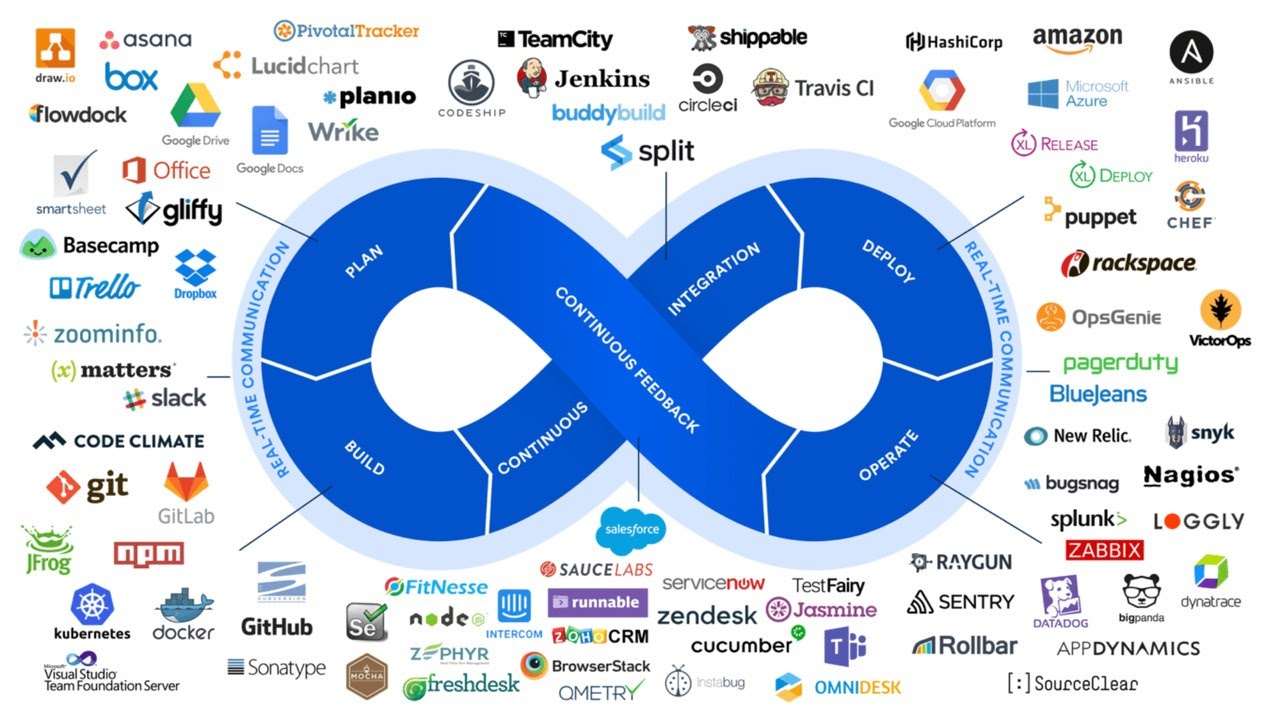
\includegraphics[width=\textwidth]{Graphics/devops}
\caption{\ac{DevOps} \cite{uplink:2021}}
\label{fig:schleife}
\end{figure}

Zu den Aufgaben des Developments auf der linke Seite in \autoref{fig:schleife} gehört das Planen (Architektur, neue Features usw.) und Bauen (Implementieren, Compilieren) der Software, wonach dann im Zusammenspiel mit den Operations eine \glqq continuous Integration\grqq\ stattfindet, also die Übergabe des Produktes von Dev zu Ops. Die Aufgaben der Operations beinhalten \glqq Deploy\grqq , also das Einsetzen bzw. Aufstellen der Software im Hardwarebereich sowie \glqq operate\grqq , womit das Benutzen der Software im gewollten Bereich gemeint ist. Als letzten Schritt wird hier das \glqq continuous Feedback\grqq\ genannt, welches wieder im Zusammenspiel mit der Abteilung des Development stattfindet. Sobald das Feeback beim Development angekommen ist, beginnt der Zyklus wieder von vorne mit der Planung und dem Bauen auf Seiten des Developments. Dargestellt durch die hellblaue Linie, die in \autoref{fig:schleife} die Schleife komplett einschließt, ist die kontinuierliche Kommunikation in Echtzeit. Jeder einzelne dieser Teilschritte wird in Kommunikation mit der jeweils anderen Abteilung abgearbeitet, es werden ständig Informationen ausgetauscht und Feedback eingeholt.

Die Tools, die um die Schleife herum in \autoref{fig:schleife} zu sehen sind, sind Beispiele für Programme, Methoden und Werkzeuge, die in den jeweiligen Schritten des \ac{DevOps}-Prozesses helfen können.

Ein wichtiger Punkt im Zuge des \ac{DevOps} ist auch die Etablierung von Fehlerkulturen, also das Akzeptieren von und Lernen aus Fehlern im Gegensatz zur Schuldzuweisung und den Versuchen, Verantwortung anderen anzuhängen. Mehr dazu jedoch in \autoref{chap:fehler}.

\section{CALMS}\label{sec:calms}



\section{Guiding Tools}